\section{Analysis of the Lockin Method}
For the analysis the 'Nulldurchgang' of both the Lock-In and the sawtooth signal needs to be calculated. First of all the slopes of the measured sawtooth were fitted with a linear fit of the form $f(x)=m\cdot x+b$. For the fit \verb|curve_fit| of the python package \verb|scipy.optimize| \cite{SciPy_Opti} was used. With these parameters the 'Nulldurchgang' for each measurement can be calculated. To do so equation \ref{Nulldurchgang1} was used, with $d_s$ being the position were the curve crosses zero. The error $\sigma_{d_s}$ is calculated using Gaussian error propagation.
\begin{equation}
	d_S=-\frac{b}{m}
	\label{Nulldurchgang1}
\end{equation}
\begin{equation}
	\sigma_{d_S}=\sqrt{(\frac{\sigma_{b}}{m})^2+(\frac{b}{m^2}\sigma_{m})^2}
\end{equation}
The parameters and 'Nulldurchgang' are documented in table \ref{SägezahnParameter}. The figures of the measured signals as well as the corresponding fits can be seen for the data of the CSV file \verb|lockin_9| in figure \ref{Example}. The other ones can be found in the appendix in figure \ref{Lock2} to \ref{Lock7}.\par
\begin{figure}[ht]
	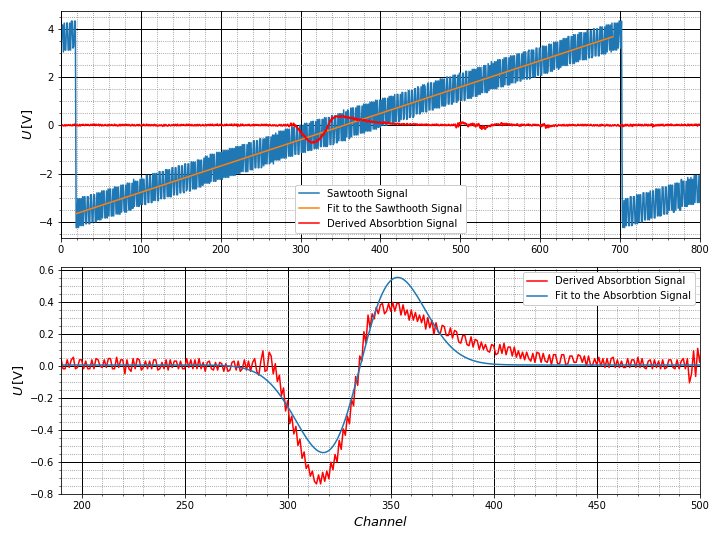
\includegraphics[scale=0.5]{Bild/LockIn8.png}
	\centering
	\caption[Plots and Fits of Lock-In Method 1]{\small The upper figure shows the data of the sawtooth in blue with the corresponding fit in orange. The absorption signal is in red. The lower one shows the part of the absorption signal which is of interest with the fit in blue.}
	\label{Example}
\end{figure}
For the high frequency signal (HF) of the NMR Oscillator the derivative of an inverse Gaussian curve was fitted. The form can be seen in eq.\ref{gaussian_ab}.
\begin{equation}
	f(x)=\frac{a(x-d_{A})e^{-\frac{(x-d_{A})^2}{2c^2}}}{c^2}+h
	\label{gaussian_ab}
\end{equation}
As can be seen in figure \ref{Example} the fits aren't very similar to the measured data. The main problem is the asymmetry of the amplitudes which are different for the data but are expected to be similar in eq.\ref{gaussian_ab}. The reason for this is very likely the Lock-In method as well as relaxation processes duo to which the expected Gaussian derivative is not a perfect match. The reason this fit was still used is that the needed parameter $d_{A}$ which gives the 'Nullstelle' isn't affected to much. This can also be seen in table \ref{GaussianTable} since here the errors on the listed parameters $d_A$, which give the needed 'Nullstellen' position, aren't to high.\par
With those two positions of the sawtooth as well as the absorption signal the distance $\Delta d$ between those can be calculated and depicted together with the corresponding frequency of the NMR Oscillator. The error for this gab $\sigma_{\Delta d}$ is calculated using eq.\ref{Gab}. 
\begin{equation}
	\sigma_{\Delta d}=\sqrt{(d_A\sigma_{dS})^2+(d_S\sigma_{dA})^2}
	\label{Gab}
\end{equation}
The data points were than fitted with the linear form $f(x)=m_2\cdot x+b_2$. The difference to the sawtooth fit is, that the error $\sigma_{\Delta d}$ was used for this fit. Since \verb|curve_fit| only takes errors of the y-axis, the errors for the frequency weren't used since they aren't as dominant for the calculation. The data points and the fit are shown in figure \ref{Nullstellenfit}. The data points coloured in green were excluded from the fit calculation. The reason for this is warming up of the magnets and the long time between the measurement of these two points and the others. This caused a slow shifting in the magnetic field and with that a shift in the resonance frequency.\par
\begin{figure}[h]
	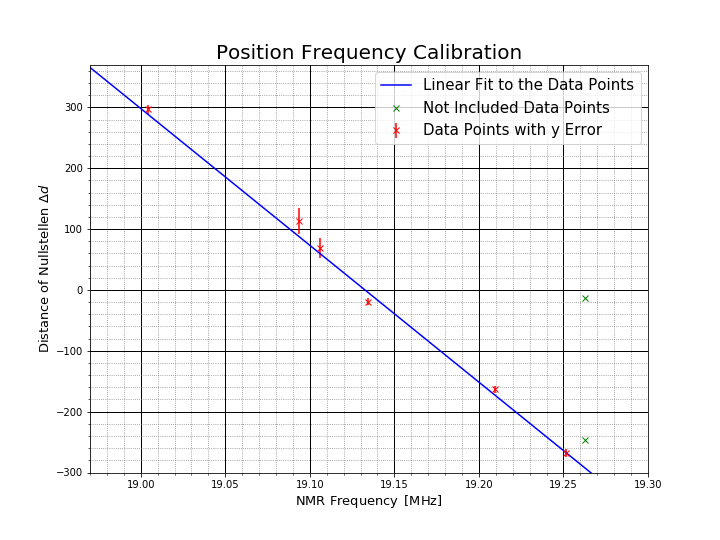
\includegraphics[scale=0.5]{Bild/Eichung.png}
	\centering
	\caption[Distance of 'Nullstellen' to Frequency Plot]{Plot of frequency against the distance $\Delta d$. The green data points were excluded from the fit calculation. The fit itself is calculated with the errors $\sigma_{\Delta d}$.}
	\label{Nullstellenfit}
\end{figure}
With the help of this fit the resonance frequency at which both 'Nullstellen' align can be found, since here the value for $\Delta d$ is zero. Using equation \ref{Nullstelle2} the frequency and its error were calculated.
\begin{equation}
f_{LockIn}=-\frac{b_2}{m_2}
\label{Nullstelle2}
\end{equation}
\begin{equation}
\sigma_{d_S}=\sqrt{(\frac{\sigma_{b}}{m})^2+(\frac{b}{m^2}\sigma_{m})^2}
\end{equation}
The resonance frequency for the Lock-In method we get using this calculation is:$$f_{LockIn}=(19.1\pm0.6)\,\text{MHz}$$
The corresponding magnetic field is calculated using the mean of the measured magnetic fields while the error is calculated using equation \ref{error Mean}.
\begin{equation}
	\sigma_x=\sqrt{\frac{1}{1-n}\sum_{n}^{i=1}(x_i-\bar{x})^2}
	\label{error Mean}
\end{equation}
Here the first 3 measured B-fields were excluded. The reason for the first two is similar to the excluded data points in fig.\ref{Nullstellenfit}. The third one was excluded duo to its huge difference to the other values. The reason the difference is either that the sawtooth wasn't turned off, or the hall sensor was to long inside the magnetic field which increased the temperature. The problems with the Hall sensor are discussed in the conclusion. With that the magnetic field is at:
$$B_{LockIn} = (463.0\pm0.7)\,\text{mT}$$
